\documentclass[]{article}
\usepackage{amsmath}
	\numberwithin{equation}{section}
	\DeclareMathOperator{\arth}{arth}
\usepackage[colorlinks=true]{hyperref}
\usepackage[magyar]{babel}
\usepackage[T1]{fontenc}
\usepackage[utf8]{inputenc}
\usepackage{graphicx}
\usepackage{geometry}
\usepackage{anysize}
\usepackage{float}
\usepackage{physics}
\usepackage{slashed}
\marginsize{10mm}{10mm}{10mm}{10mm}
\newcommand\at[2]{\left.#1\right|_{#2}}


%opening
\title{Szoftvertechnikák 1. HF}
\author{Németh Márton}

\begin{document}

\maketitle

\section{Docker használata}

\subsection{Docker telepítése}

\texttt{pacman -S docker}
\subsection{Docker image}

A fájlrendszer és a paraméterek összessége. Rétegekből épül fel, ezek az image létrehozása után csak olvashatóak.

\subsection{Docker container}
Amikor az image-et containerré alakítjuk (pl. \texttt{docker run}), akkor a docker egy írható/olvasható réteget helyez a csak olvasható rétegek felé.

\subsection{Dockerfile}

A dockerfile egy image leírását tartalmazza. Ez alapján a docker el tud készíteni egy image-et.

\section{Container vs VM}

\begin{figure}
	\centering
	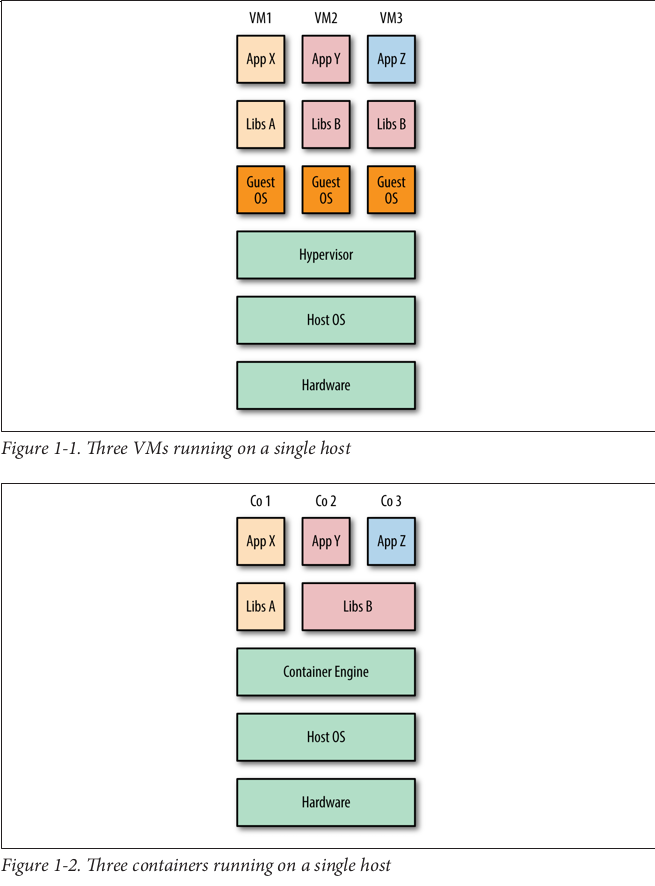
\includegraphics[width=0.7\linewidth]{cont_vs_vm}
	\caption{}
	\label{fig:contvsvm}
\end{figure}

\section{Példák docker futtatására}

\subsection{Hello World}

\texttt{docker run debian echo "Hello World"}

Ez a parancs futtatja a debian image-et, azon belül elindítja az echo programot, ami kiírja, hogy "Hello World".

\subsection{Két docker container kommunikációja}

Az első parancs elindítja a redis containert a háttérben, és elnevezi "myredis"-nek:

\texttt{docker run --name myredis -d redis}

A következő parancs elindít még egy redis containert. A link kapcsoló segítségével összekapcsolhatjuk a két containert, így a második container "redis" néven látja az elsőt. Ezt úgy éri el, hogy a \texttt{/etc/hosts} fájlba beírja az első, háttérben futó container IP-címét. A containerben elindul egy bash shell, itt a megfelelő parancsokat kiadva tudunk kommunikálni a másik containerrel.

\texttt{docker run --rm -it --link myredis:redis redis /bin/bash}

\begin{figure}
	\centering
	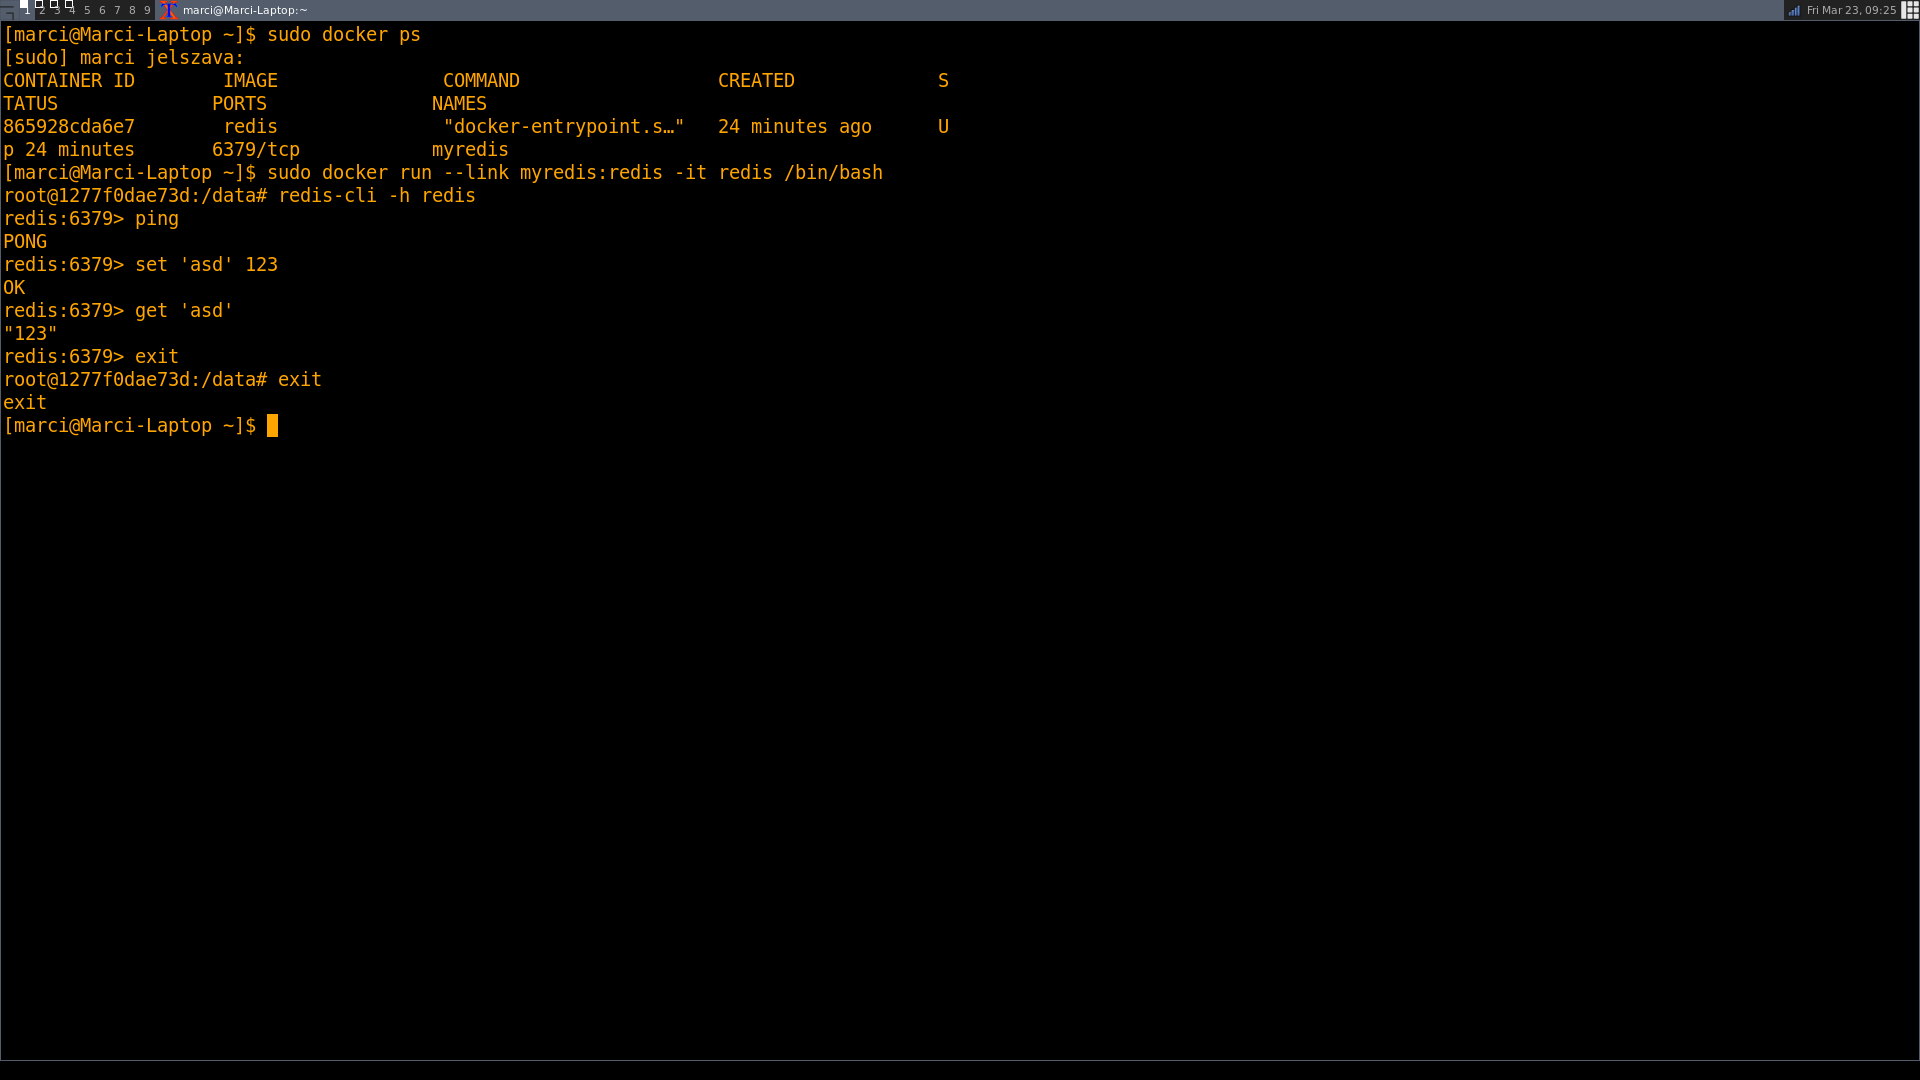
\includegraphics[width=0.7\linewidth]{redis.png}
	\caption{}
	\label{fig:redis}
\end{figure}


\end{document}
